\documentclass{beamer}
\usepackage{verbatim}
\usepackage{xcolor}
\usepackage{multirow}
%\usepackage{enumitem}
\usetheme{Warsaw}
\setbeamertemplate{navigation symbols}{}
\newcommand{\blue}[1]{{\color{blue} #1}}
\newcommand{\red}[1]{{\color{red} #1}}
\newcommand{\grn}[1]{{\color{green} #1}}
\newcommand{\bluRed}[2]{{\color{blue} #1}{\color{red} #2}}
\newcommand{\qtns}[0]{\begin{center} Questions? \end{center}}
\newcommand{\nl}[1]{\vspace{#1 em}}
\newcommand{\cntrImg}[2]{\begin{center}\includegraphics[scale=#2]{#1}\end{center}}
\newcommand{\defn}[1]{{\bf #1}}

\title{Math 3070, Applied Statistics}

\begin{document}

\begin{frame}
    \begin{beamercolorbox}[rounded=true,wd=\textwidth,center]{title}
        \usebeamerfont{title}\inserttitle
    \end{beamercolorbox}
    \begin{center}
        Section 1\\
        \nl{0.5}
        August 21, 2019
    \end{center}

\end{frame}

\begin{frame}{Lecture Outline, 8/21}
    \begin{itemize}
        \item 1.2 Outliers
        \item 1.3 Measures of Location (Center)
        \item 1.4 Measures of Spread (Variability)
    \end{itemize}
\end{frame}

\begin{frame}{Outliers, Section 1.2}
    \defn{Outlier}: Value which is significantly different from other observations. Mathematical definitions may vary.
    \begin{center}
        Example: 8,3,2,5,4,2,3,5,3,2,1,5,7,7,8,8,9,99,101\\
        \nl{0.5}
        Outliers: 99 and 101
    \end{center}
    \qtns
\end{frame}

\begin{frame}{Measures of Location and Spread, Preface}
    \begin{itemize}
        \item {\bf Population parameters}: describe features of the population. Examples: population mean $\mu$, variance $\sigma^2$ and standard deviation $\sigma$.
        \item {\bf Sample statistics }: describe features of a sample. Examples: sample mean $\overline{x}$, variance $s^2$ and standard deviation $s$.
    \end{itemize}
\end{frame}

\begin{frame}{Measures of Location (Section 1.3)}
    Goal: Find the center or "middle" of the data.
    \nl{1}\\
    Tools: \defn{Sample Mean}, \defn{Sample Median} and \defn{Trimmed Mean}
    \nl{1}\\
    Consideration: outliers
\end{frame}

\begin{frame}{Sample Mean, Definition}
    Given a set of data denoted as $x_1, x_2, \ldots, x_n$. \\
    Note, sample size = $n$.\\
    \nl{1}
    {\bf Sample Mean:}
    $$\overline{x} = \frac1n\sum_{i=1}^n x_i = \frac{x_1+\cdots+x_n}n$$
\end{frame}

\begin{frame}{Sample Mean, Example (no outlier)}
    Data: 8,3,2,5,4,2,3\\
    \nl{0.5}
    With previous notation, \blue{$x_1=8, x_2 =3, x_3 = 2, \ldots, x_7 = 3$}.\\
    \nl{0.5}
    \red{Sample Size = n = 7}
    \[\overline{x} = \frac{\sum_{i=1}^n \blue{x_i}}{\red{n}} = \frac{\blue{8+3+2+5+4+2+3}}{\red{7}} = \frac{\blue{27}}{\red{7}} \approx 3.86\]
\end{frame}

\begin{frame}{Sample Mean, Example (one outlier)}
    Data: 8,3,2,5,4,2,300\\
    \nl{0.5}
    With previous notation, \blue{$x_1=8, x_2 =3, x_3 = 2, \ldots, x_7 = 300$}.\\
    \nl{0.5}
    \red{Sample Size = n = 7}
    \[\overline{x} = \frac{\blue{8+3+2+5+4+2+300}}{\red{7}} = \frac{\blue{324}}{\red{7}} \approx 46.28\]
\end{frame}

\begin{frame}{Sample Mean, Comments and Questions}
    \begin{itemize}
        \item Sample mean is measure of center. 
        \item Important since it estimates the population mean, used extensively in population models.
        \item Same units as data.
        \item Sensitive to outliers. Few large values can pull the sample mean towards their direction.
    \end{itemize}
    \qtns
\end{frame}

\begin{frame}{Sample Median, Definition and Method}
    Given a set of data denoted as $x_1, x_2, \ldots, x_n$. \\
    Note, sample size = $n$.\\
    \nl{1}
    {\bf Sample Median:}
    $$\tilde{x} = \begin{cases}
            x_{(n+1)/2}                 & \text{if $n$ is odd}  \\
            \frac12(x_{n/2} +x_{n/2+1}) & \text{if $n$ is even}
        \end{cases}$$
    \begin{enumerate}
        \item  Sort the data from smallest to largest.
        \item If $n$ is odd, then the sample median $\tilde{x}$ is the middle observation in the list; if $n$ is even, then $\tilde{x}$ is the average of the two middle observations.
    \end{enumerate}
\end{frame}

\begin{frame}{Sample Median, Example (no outlier)}
    Data: 8,3,2,5,4,2,3\\
    \nl{0.5}
    Sorted Data: 2,2,3,3,4,5,8\\
    \nl{0.5}
    \[\tilde{x} = 3\]
\end{frame}

\begin{frame}{Sample Median, Example (one outlier)}
    Data: 8,3,2,5,4,2,300\\
    \nl{0.5}
    Sorted Data: 2,2,3,4,5,8,300\\
    \nl{0.5}
    \[\tilde{x} = 4\]
\end{frame}

\begin{frame}{Sample Median, Comments and Questions}
    \begin{itemize}
        \item Sample median is measure of center.
        \item Not sensitive to outliers or {\bf robust}.
        \item Same units as data.
        \item If $\overline{x}$ is much further right than $\tilde{x}$ ($\overline{x}>\tilde{x}$), then outliers may be pulling the mean to the right. In this case, the distribution is likely right-skewed. Likewise, if $\overline{x}$ is much further left than $\tilde{x}$, the distribution is likely left-skewed.
    \end{itemize}
    \qtns
\end{frame}

\begin{frame}{Trimmed Mean, Definition and Method}
    Median is robust, but sample mean estimates the mean, an important probabilistic quantity. {\bf Trimmed Means} are more robust, but behave similiar to sample means.\\
    \nl{0.5}
    Given a set of data denoted as $x_1, x_2, \ldots, x_n$. \\
    \nl{0.5}
    \begin{enumerate}
        \item Order the data, smallest to largest.
        \item Discard the largest and smallest $\alpha \%$, $\alpha$ to be chosen.
        \item Compute the mean of the remaining numbers. This is the trimmed mean, $\overline{x}_\alpha$
    \end{enumerate}
\end{frame}

\begin{frame}{Trimmed Mean, Example (no outlier)}
    Data: 1,8,3,2,5,4,2,3\\
    \nl{0.5}
    Sorted Data: \red{1},\blue{2,2,3,3,4,5},\red{8}\\
    \nl{0.5}
    For $\alpha =12$ (the $12\%$ trimmed mean),  the \red{first} and \red{last} numbers are \red{discarded}. The \blue{remaining} are \blue{averaged}.

    \[\overline{x}_{12} = \frac{\blue{2+2+3+3+4+5}}{6} \approx 3.16\]

    \[\tilde{x} = (3+3)/2=3,\hskip 1em \overline{x} =3.5\]
\end{frame}

\begin{frame}{Trimmed Mean, Example (one outlier)}
    Data: 1,8,3,2,5,4,2,300\\
    \nl{0.5}
    Sorted Data: \red{1},\blue{2,2,3,3,4,8},\red{300}\\
    \nl{0.5}
    For $\alpha =12$,  the \red{first} and \red{last} numbers are \red{discarded}. The \blue{remaining} are \blue{averaged}.

    \[\overline{x}_{12} = \frac{\blue{2+2+3+3+4+8}}{6} \approx 3.66\]

    \[\tilde{x} = (3+3)/2=3,\hskip 1em \overline{x} = 40.625\]
\end{frame}

\begin{frame}{Trimmed Mean, Comments and Questions}
    \begin{itemize}
        \item Trimmed mean is measure of center.
        \item Can be robust depending on $\alpha$.
        \item Not clear how to pick $\alpha$.
    \end{itemize}
    \qtns
\end{frame}

\begin{frame}{Measures of Spread (Section 1.4)}
    Goal: Find the spread or variability of the data.
    \nl{1}\\
    Tools: \defn{Sample Variance and Standard Deviation}, \defn{Range} and \defn{Interquartile Range} (IQR or the 'fourth spread' in the book), box plots
    \nl{1}\\
    Consideration: outliers
\end{frame}

\begin{frame}{Sample Variance, Standard Deviation and Range, Definition}
    Given a set of data denoted as $x_1, x_2, \ldots, x_n$. \\
    \nl{0.5}
    $n=\mbox{sample size}$\\
    \nl{0.5}
    \[\mbox{\bf{Range}} := \max(x_i) - \min(x_i)\]
    \[\mbox{\bf{Sample Variance}} := s^2 = \frac{\sum_{i=1}^n (x_i - \overline{x})^2}{n-1} = \frac{S_{xx}}{n-1}\]
    \[\mbox{\bf{Sample Standard Deviation}} := s = \sqrt{s^2}\]
    \begin{center}
        $s^2$ and $s$ are important since the estimate population variance and standard deviation. Again, used in probabilistic models.
    \end{center}
    \begin{center}
    $\overline{x}$ is in the definition of $s^2$ and $s$, shouldn't expect them to be robust. And, the Range depends solely depends on the value of the outliers, shouldn't expect it to be robust either.
    \end{center}
\end{frame}

\begin{frame}{Sample Variance, Standard Deviation and Range, Example (no outlier)}
    Data: \blue{1,8,3,2,5,4,2,3}\\
    \nl{0.5}
    Range $= 8-1 =7$\\
    \nl{0.5}
    sample size = $\grn{8}$, $\red{\overline{x} =3.5}$ from eariler
    \[s^2 = \frac{\sum_{i=1}^n (\blue{x_i} - \red{3.5})^2}{\grn{8}-1} \approx 4.85\]
    \[s = \sqrt{s^2} \approx 2.2\]
\end{frame}

\begin{frame}{Sample Variance, Standard Deviation and Range, Example (one outlier)}
    Data: \blue{1,8,3,2,5,4,2,300}\\
    \nl{0.5}
    Range $= 300-1 =299$\\
    \nl{0.5}
    sample size = $\grn{8}$, $\red{\overline{x} =40.625}$ from eariler
    \[s^2 = \frac{\sum_{i=1}^n (\blue{x_i} - \red{40.625})^2}{\grn{8}-1} \approx 10,989\]
    \[s = \sqrt{s^2} \approx 104.83\]
\end{frame}

\begin{frame}{Sample Variance, Standard Deviation and Range, Comments and Questions}
    \begin{itemize}
        \item Sample Variance, Standard Deviation and Range are sensitive to outliers.
        \item Sample variance is measured in squared units while range and standard deviation have the same units as the data.
    \end{itemize}
    \qtns
\end{frame}

\begin{frame}{Interquartile Range, Method}
    Given a set of data denoted as $x_1, x_2, \ldots, x_n$. \\
    \begin{enumerate}
        \item Separate the data into the lower half and upper half.\\
        (Include the median $\tilde{x}$ in both halves if $n$ is odd.)
        \item The median of the lower half is called the {\bf first quartile}, or lower fourth.
        \item The median of the higher half is called the {\bf third quartile}, or upper fourth. 
        \item Their difference is the {\bf interquartile range} (IQR), or fourth spread:
        $$\text{IQR} = \text{third quartile}-\text{first quartile}$$
        \end{enumerate}
\end{frame}

\begin{frame}{Interquartile Range, Example (no outlier)}
    Data: 1,8,3,2,5,4,2,3,7\\
    Sorted Data: 1,2,2,3,3,4,5,7,8\\
    Step 1: Separate the data into the lower half and higher half.\\
    \begin{center}
    \red{ Lower Half: 1,2,2,3,3} \hskip 2em \blue{Upper Half:  3,4,5,7,8}
    \end{center}
    Steps 2 and 3: median of \blue{upper half} is the \blue{third quartile}; median of \red{lower half} is the \red{first quartile}\\
    \begin{center}
        \red{first quartile $ = 2$} \hskip 2em \blue{third quartile $ = 5$}
    \end{center}
    Step 4: Positive difference is the IQR
    \[\text{IQR} = \blue{5} - \red{2} = 3\]
\end{frame}

\begin{frame}{Interquartile Range, Example (one outlier)}
    Data: 1,8,3,2,5,4,2,3,799\\
    Sorted Data: 1,2,2,3,3,4,5,8,799\\
    Step 1: Separate the data into the smaller half and larger half.\\
    \begin{center}
    \red{ Lower Half: 1,2,2,3,3} \hskip 2em \blue{Upper Half:  3,4,5,8,799}
    \end{center}
    Steps 2 and 3: median of \blue{upper half} is the \blue{third quartile}; median of \red{lower half} is the \red{first quartile}\\
    \begin{center}
    \red{first quartile $ = 2$} \hskip 2em \blue{third quartile $ = 5$}
    \end{center}
    Step 4: Positive difference is the IQR
    \[\text{IQR} = \blue{5} - \red{2} = 3\]
\end{frame}

\begin{frame}{Sample Variance, Standard Deviation and Range, Comments and Questions}
    \begin{itemize}
        \item IQR is a robust measure of spread.
        \item IQR has the same units as the data.
    \end{itemize}
    \qtns
\end{frame}

\begin{frame}{Measures of Location and Spread, Summary}
    \begin{itemize}
        \item Sample mean and median are measures of location. 
        \item Median is robust; mean is not.
        \item Mean $<<$ median indicates likely left-skew. Mean $>>$ median indicates likely right-skew.
        \item Sample variance, standard deviation, IQR and range are measures of spread. 
        \item Only the IQR is robust.
        \item $\overline{x}$, $s^2$ and $s$ are important estimators of population parameters which will impact probabilistic models.
    \end{itemize}
\end{frame}

\begin{frame}{Linear Transformations}
    Goal: Relate the sample mean, variance and standard deviation of data after linear transformations, scaling then shifting (ax +c).
\end{frame}

\begin{frame}{Linear Transformations and the Sample Mean}
    Given data, $x_1, x_2, \ldots, x_n$
    \begin{center}
        Linearly transform the data: $y_i = a x_i+c$. $a,c$ are constants.
    \end{center}
    Relate the sample means of each data.
    \[\overline{y} = \frac{(\sum_{i=1}^n ax_i +c)}{n} = \frac{(\sum_{i=1}^n ax_i)+ (\sum_{i=1}^nc)}{n} = \frac{a(\sum_{i=1}^n x_i)+ nc}{n}\]
    \[ = \frac{a\sum_{i=1}^n x_i}{n} + \frac{nc}{n} = a\frac{\sum_{i=1}^n x_i}{n} + c = a\overline{x} + c\]
    \[\overline{y} = a \overline{x} + c\]
    Linearly transformations of data transform the mean in the exact same way.
\end{frame}

\begin{frame}{Linear Transformations and the Sample Variance and Standard Deviation}
    Given data, $x_1, x_2, \ldots, x_n$
    \begin{center}
        Linearly transform the data: $y_i = a x_i+c$. $a,c$ are constants.
    \end{center}
    The sample mean of both data is related, $\blue{\overline{y}=a\overline{x} + c}$.\\
    Relate the variances of each data, $s^2_y$ and $s_x^2$.
    \[s_y^2 = \frac{\sum_{i=1}^n (y_i - \blue{\overline{y}})^2}{n-1} = \frac{\sum_{i=1}^n (a x_i +c - \blue{(a \overline{x} + c)})^2}{n-1}\]
    \[= \frac{\sum_{i=1}^n a^2 ( x_i - \blue{\overline{x} })^2}{n-1} = a^2 s_x^2\]
    \[s_y^2 = a^2 s_x^2, \hskip 1em s_y = |a| s_x \]
    Sample variance and standard deviation ignore shifts. Variance squares scales as the square of the scaling and standard deviation scales by the absolute value.
\end{frame}

\begin{frame}{Linear Transformations, Summary}
    Given data, $x_1, x_2, \ldots, x_n$, if the data is is linearly transformed: $y_i = a x + c$, $a,c$ are constants, then the following hold.
    \begin{itemize}
        \item $\overline{y} = a \overline{x} + c$
        \item $s_y^2 = a^2 s_x^2$
        \item $s_y = |a| s_x$
    \end{itemize}
\end{frame}

\begin{frame}{Linear Transformations, Example}
    Denote the previous data, $1,8,3,2,5,4,2,3$ by $x_i$. The sample mean, variance and standard deviation were calculated and will be denoted as \[\overline{x} = 3.5, s_x^2 \approx 4.85 \mbox{ and } s_x \approx 2.2.\]
    Multiply the data by $\blue{-2}$ and add $\red{100}$, $y_i = \blue{-2}x_i +\red{100}$.
    \[\overline{y} = \blue{-2}\overline{x} + \red{100} = \blue{-2}(3.5) + \red{100} = 93\]
    \[s_y^2 = (\blue{-2})^2 s_x^2 \approx 4(4.85) = 19.4\]
    \[s_y = |\blue{-2}| s_x \approx 2(2.2) = 4.4\]
\end{frame}

\begin{frame}{Linear Transformations, Comments and Questions?}
    \begin{itemize}
        \item May not work with other transformations.
        \item Formulas will be paralleled in probabilistic models.
    \end{itemize}
    \qtns
\end{frame}

\begin{frame}{Five-number summary and Boxplot}
    \begin{tabular}{p{2.5in}p{2in}}
    \begin{tabular}{p{2.5in}}
        Five-number summary
    \begin{enumerate}
    \item Minimum observation
    \item First quartile %lower fourth
    \item Median
    \item Third quartile %upper fourth
    \item Maximum observation
    \end{enumerate}
    For the concrete strength data: 
    $$5.90, 7.00, 7.70, 8.85, 11.80$$
    
    This is shown graphically in a Boxplot: The bottom and top of the box show the first and third quartiles; the horizontal line inside the box shows the median; the whiskers (dotted lines) extend to the minimum and maximum observations.
    \end{tabular} &
    \begin{tabular}{p{2in}}
    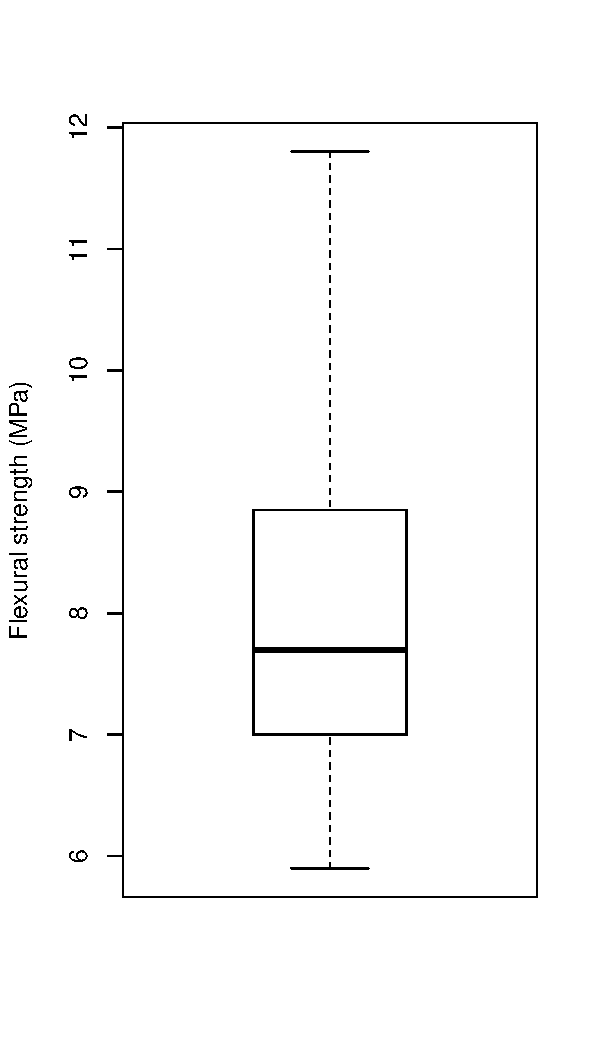
\includegraphics[scale=.4]{ch01_strength_boxplot.pdf}
    \end{tabular}
    \end{tabular}
\end{frame}

\begin{frame}{Sample Proportion, Definition}
    Goal: Estimate the proportion of times a specified outcome of a categorical variable is observed.

    {\bf Sucess}: Number of times a specified outcome of a categorical variable is observed.

    \[\text{\bf Sample Proportion}:= \hat{p} = \frac{\text{Successes}}{\text{Sample Size}}\]
\end{frame}

\begin{frame}{Sample Proportion, Example}
    Data: 153 heads are observed in 300 variables.
    \begin{center}
    \red{successes = 153}, \hskip 1em \blue{sample size = 304}
    \end{center}
    \[\hat{p} =\frac{\red{153}}{\blue{304}} \approx 0.503\]
    The proportion of heads in the sample is roughly 0.503.
\end{frame}

\begin{frame}{Sample Proportion, Questions}
    \qtns
\end{frame}

\end{document}